\documentclass{standalone}
\usepackage{tikz}
\usetikzlibrary{patterns, positioning}


\begin{document}
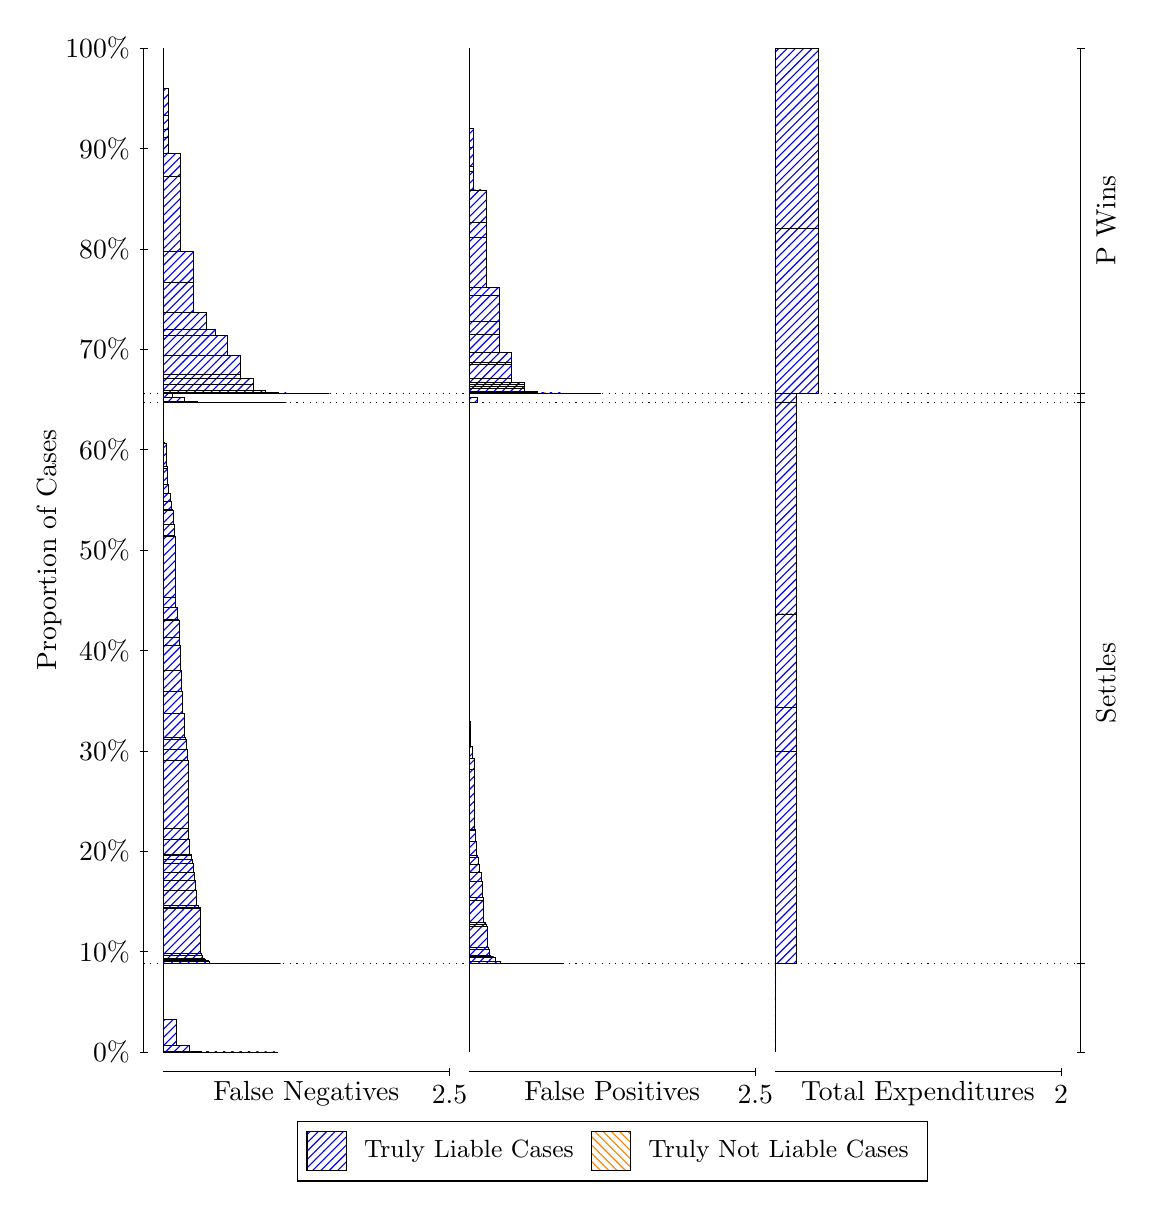
\begin{tikzpicture}
\draw[black, very thin] (1.5,1.75) -- (1.5,14.5);
\node[rotate=90, text=black, anchor=center] at (0.3, 8.125) {Proportion of Cases};
\draw[black, very thin] (1.45,1.75) -- (1.55,1.75);
\node[text=black, anchor=east] at (1.45, 1.75) {0\%};
\draw[black, very thin] (1.45,3.025) -- (1.55,3.025);
\node[text=black, anchor=east] at (1.45, 3.025) {10\%};
\draw[black, very thin] (1.45,4.3) -- (1.55,4.3);
\node[text=black, anchor=east] at (1.45, 4.3) {20\%};
\draw[black, very thin] (1.45,5.575) -- (1.55,5.575);
\node[text=black, anchor=east] at (1.45, 5.575) {30\%};
\draw[black, very thin] (1.45,6.85) -- (1.55,6.85);
\node[text=black, anchor=east] at (1.45, 6.85) {40\%};
\draw[black, very thin] (1.45,8.125) -- (1.55,8.125);
\node[text=black, anchor=east] at (1.45, 8.125) {50\%};
\draw[black, very thin] (1.45,9.4) -- (1.55,9.4);
\node[text=black, anchor=east] at (1.45, 9.4) {60\%};
\draw[black, very thin] (1.45,10.675) -- (1.55,10.675);
\node[text=black, anchor=east] at (1.45, 10.675) {70\%};
\draw[black, very thin] (1.45,11.95) -- (1.55,11.95);
\node[text=black, anchor=east] at (1.45, 11.95) {80\%};
\draw[black, very thin] (1.45,13.225) -- (1.55,13.225);
\node[text=black, anchor=east] at (1.45, 13.225) {90\%};
\draw[black, very thin] (1.45,14.5) -- (1.55,14.5);
\node[text=black, anchor=east] at (1.45, 14.5) {100\%};

\draw[black, very thin] (13.4,1.75) -- (13.4,14.5);
\draw[black, very thin] (13.35,1.75) -- (13.45,1.75);
\node[anchor=west] at (13.35, 1.75) {};
\draw[black, very thin] (13.35,2.872) -- (13.45,2.872);
\node[anchor=west] at (13.35, 2.872) {};
\draw[black, very thin] (13.35,10.001) -- (13.45,10.001);
\node[anchor=west] at (13.35, 10.001) {};
\draw[black, very thin] (13.35,10.118) -- (13.45,10.118);
\node[anchor=west] at (13.35, 10.118) {};
\draw[black, very thin] (13.35,14.5) -- (13.45,14.5);
\node[anchor=west] at (13.35, 14.5) {};

\draw[black, very thin, pattern color=blue, pattern=north east lines] (1.75,1.75) rectangle (3.2033,1.75);
\draw[black, very thin, pattern color=blue, pattern=north east lines] (1.75,1.75) rectangle (3.0419,1.75);
\draw[black, very thin, pattern color=blue, pattern=north east lines] (1.75,1.75) rectangle (2.8804,1.75);
\draw[black, very thin, pattern color=blue, pattern=north east lines] (1.75,1.75) rectangle (2.7189,1.75);
\draw[black, very thin, pattern color=blue, pattern=north east lines] (1.75,1.75) rectangle (2.5574,1.75);
\draw[black, very thin, pattern color=blue, pattern=north east lines] (1.75,1.75) rectangle (2.3959,1.7503);
\draw[black, very thin, pattern color=blue, pattern=north east lines] (1.75,1.7503) rectangle (2.2344,1.7579);
\draw[black, very thin, pattern color=blue, pattern=north east lines] (1.75,1.7579) rectangle (2.073,1.8357);
\draw[black, very thin, pattern color=blue, pattern=north east lines] (1.75,1.8357) rectangle (1.9115,2.1659);
\draw[black, very thin, pattern color=orange, pattern=north west lines] (1.75,2.1659) rectangle (1.75,2.1659);
\draw[black, very thin, pattern color=blue, pattern=north east lines] (1.75,2.1659) rectangle (1.75,2.872);
\draw[black, very thin, pattern color=blue, pattern=north east lines] (1.75,2.872) rectangle (3.2397,2.872);
\draw[black, very thin, pattern color=blue, pattern=north east lines] (1.75,2.872) rectangle (3.167,2.872);
\draw[black, very thin, pattern color=blue, pattern=north east lines] (1.75,2.872) rectangle (3.0943,2.872);
\draw[black, very thin, pattern color=blue, pattern=north east lines] (1.75,2.872) rectangle (3.0782,2.872);
\draw[black, very thin, pattern color=blue, pattern=north east lines] (1.75,2.872) rectangle (3.0217,2.872);
\draw[black, very thin, pattern color=blue, pattern=north east lines] (1.75,2.872) rectangle (3.0055,2.872);
\draw[black, very thin, pattern color=blue, pattern=north east lines] (1.75,2.872) rectangle (2.949,2.872);
\draw[black, very thin, pattern color=blue, pattern=north east lines] (1.75,2.872) rectangle (2.9329,2.872);
\draw[black, very thin, pattern color=blue, pattern=north east lines] (1.75,2.872) rectangle (2.9167,2.872);
\draw[black, very thin, pattern color=blue, pattern=north east lines] (1.75,2.872) rectangle (2.8763,2.872);
\draw[black, very thin, pattern color=blue, pattern=north east lines] (1.75,2.872) rectangle (2.8602,2.872);
\draw[black, very thin, pattern color=blue, pattern=north east lines] (1.75,2.872) rectangle (2.844,2.872);
\draw[black, very thin, pattern color=blue, pattern=north east lines] (1.75,2.872) rectangle (2.8037,2.872);
\draw[black, very thin, pattern color=blue, pattern=north east lines] (1.75,2.872) rectangle (2.7875,2.872);
\draw[black, very thin, pattern color=blue, pattern=north east lines] (1.75,2.872) rectangle (2.7714,2.872);
\draw[black, very thin, pattern color=blue, pattern=north east lines] (1.75,2.872) rectangle (2.7552,2.872);
\draw[black, very thin, pattern color=blue, pattern=north east lines] (1.75,2.872) rectangle (2.731,2.872);
\draw[black, very thin, pattern color=blue, pattern=north east lines] (1.75,2.872) rectangle (2.7149,2.872);
\draw[black, very thin, pattern color=blue, pattern=north east lines] (1.75,2.872) rectangle (2.6987,2.872);
\draw[black, very thin, pattern color=blue, pattern=north east lines] (1.75,2.872) rectangle (2.6826,2.872);
\draw[black, very thin, pattern color=blue, pattern=north east lines] (1.75,2.872) rectangle (2.6583,2.872);
\draw[black, very thin, pattern color=blue, pattern=north east lines] (1.75,2.872) rectangle (2.6422,2.872);
\draw[black, very thin, pattern color=blue, pattern=north east lines] (1.75,2.872) rectangle (2.626,2.872);
\draw[black, very thin, pattern color=blue, pattern=north east lines] (1.75,2.872) rectangle (2.6099,2.872);
\draw[black, very thin, pattern color=blue, pattern=north east lines] (1.75,2.872) rectangle (2.5937,2.872);
\draw[black, very thin, pattern color=blue, pattern=north east lines] (1.75,2.872) rectangle (2.5857,2.872);
\draw[black, very thin, pattern color=blue, pattern=north east lines] (1.75,2.872) rectangle (2.5695,2.872);
\draw[black, very thin, pattern color=blue, pattern=north east lines] (1.75,2.872) rectangle (2.5534,2.872);
\draw[black, very thin, pattern color=blue, pattern=north east lines] (1.75,2.872) rectangle (2.5372,2.872);
\draw[black, very thin, pattern color=blue, pattern=north east lines] (1.75,2.872) rectangle (2.5211,2.872);
\draw[black, very thin, pattern color=blue, pattern=north east lines] (1.75,2.872) rectangle (2.513,2.872);
\draw[black, very thin, pattern color=blue, pattern=north east lines] (1.75,2.872) rectangle (2.4969,2.8726);
\draw[black, very thin, pattern color=blue, pattern=north east lines] (1.75,2.8726) rectangle (2.4807,2.8728);
\draw[black, very thin, pattern color=blue, pattern=north east lines] (1.75,2.8728) rectangle (2.4646,2.8728);
\draw[black, very thin, pattern color=blue, pattern=north east lines] (1.75,2.8728) rectangle (2.4484,2.8729);
\draw[black, very thin, pattern color=blue, pattern=north east lines] (1.75,2.8729) rectangle (2.4403,2.8733);
\draw[black, very thin, pattern color=blue, pattern=north east lines] (1.75,2.8733) rectangle (2.4323,2.8733);
\draw[black, very thin, pattern color=blue, pattern=north east lines] (1.75,2.8733) rectangle (2.4242,2.8733);
\draw[black, very thin, pattern color=blue, pattern=north east lines] (1.75,2.8733) rectangle (2.408,2.8757);
\draw[black, very thin, pattern color=blue, pattern=north east lines] (1.75,2.8757) rectangle (2.3919,2.8763);
\draw[black, very thin, pattern color=blue, pattern=north east lines] (1.75,2.8763) rectangle (2.3757,2.8768);
\draw[black, very thin, pattern color=blue, pattern=north east lines] (1.75,2.8768) rectangle (2.3596,2.8772);
\draw[black, very thin, pattern color=blue, pattern=north east lines] (1.75,2.8772) rectangle (2.3515,2.8775);
\draw[black, very thin, pattern color=blue, pattern=north east lines] (1.75,2.8775) rectangle (2.3354,2.9012);
\draw[black, very thin, pattern color=blue, pattern=north east lines] (1.75,2.9012) rectangle (2.3192,2.9106);
\draw[black, very thin, pattern color=blue, pattern=north east lines] (1.75,2.9106) rectangle (2.3031,2.9173);
\draw[black, very thin, pattern color=blue, pattern=north east lines] (1.75,2.9173) rectangle (2.2869,2.9238);
\draw[black, very thin, pattern color=blue, pattern=north east lines] (1.75,2.9238) rectangle (2.2789,2.9314);
\draw[black, very thin, pattern color=blue, pattern=north east lines] (1.75,2.9314) rectangle (2.2708,2.9341);
\draw[black, very thin, pattern color=blue, pattern=north east lines] (1.75,2.9341) rectangle (2.2627,2.9343);
\draw[black, very thin, pattern color=blue, pattern=north east lines] (1.75,2.9343) rectangle (2.2466,2.9826);
\draw[black, very thin, pattern color=blue, pattern=north east lines] (1.75,2.9826) rectangle (2.2304,3.0061);
\draw[black, very thin, pattern color=blue, pattern=north east lines] (1.75,3.0061) rectangle (2.2223,3.5695);
\draw[black, very thin, pattern color=blue, pattern=north east lines] (1.75,3.5695) rectangle (2.2143,3.5909);
\draw[black, very thin, pattern color=blue, pattern=north east lines] (1.75,3.5909) rectangle (2.1981,3.6078);
\draw[black, very thin, pattern color=blue, pattern=north east lines] (1.75,3.6078) rectangle (2.19,3.6131);
\draw[black, very thin, pattern color=blue, pattern=north east lines] (1.75,3.6131) rectangle (2.1739,3.8058);
\draw[black, very thin, pattern color=blue, pattern=north east lines] (1.75,3.8058) rectangle (2.1577,3.9286);
\draw[black, very thin, pattern color=blue, pattern=north east lines] (1.75,3.9286) rectangle (2.1416,4.0351);
\draw[black, very thin, pattern color=blue, pattern=north east lines] (1.75,4.0351) rectangle (2.1254,4.1447);
\draw[black, very thin, pattern color=blue, pattern=north east lines] (1.75,4.1447) rectangle (2.1174,4.1983);
\draw[black, very thin, pattern color=blue, pattern=north east lines] (1.75,4.1983) rectangle (2.1093,4.2528);
\draw[black, very thin, pattern color=blue, pattern=north east lines] (1.75,4.2528) rectangle (2.1012,4.2552);
\draw[black, very thin, pattern color=blue, pattern=north east lines] (1.75,4.2552) rectangle (2.0851,4.4477);
\draw[black, very thin, pattern color=blue, pattern=north east lines] (1.75,4.4477) rectangle (2.0689,4.5895);
\draw[black, very thin, pattern color=blue, pattern=north east lines] (1.75,4.5895) rectangle (2.0609,5.4587);
\draw[black, very thin, pattern color=blue, pattern=north east lines] (1.75,5.4587) rectangle (2.0528,5.5974);
\draw[black, very thin, pattern color=blue, pattern=north east lines] (1.75,5.5974) rectangle (2.0366,5.7198);
\draw[black, very thin, pattern color=blue, pattern=north east lines] (1.75,5.7198) rectangle (2.0286,5.7437);
\draw[black, very thin, pattern color=blue, pattern=north east lines] (1.75,5.7437) rectangle (2.0124,6.0492);
\draw[black, very thin, pattern color=blue, pattern=north east lines] (1.75,6.0492) rectangle (1.9963,6.3293);
\draw[black, very thin, pattern color=blue, pattern=north east lines] (1.75,6.3293) rectangle (1.9801,6.5984);
\draw[black, very thin, pattern color=blue, pattern=north east lines] (1.75,6.5984) rectangle (1.964,6.9208);
\draw[black, very thin, pattern color=blue, pattern=north east lines] (1.75,6.9208) rectangle (1.9559,7.0158);
\draw[black, very thin, pattern color=blue, pattern=north east lines] (1.75,7.0158) rectangle (1.9478,7.2385);
\draw[black, very thin, pattern color=blue, pattern=north east lines] (1.75,7.2385) rectangle (1.9397,7.2437);
\draw[black, very thin, pattern color=blue, pattern=north east lines] (1.75,7.2437) rectangle (1.9236,7.3913);
\draw[black, very thin, pattern color=blue, pattern=north east lines] (1.75,7.3913) rectangle (1.9074,7.5308);
\draw[black, very thin, pattern color=blue, pattern=north east lines] (1.75,7.5308) rectangle (1.8994,8.2973);
\draw[black, very thin, pattern color=blue, pattern=north east lines] (1.75,8.2973) rectangle (1.8913,8.3129);
\draw[black, very thin, pattern color=blue, pattern=north east lines] (1.75,8.3129) rectangle (1.8913,8.4454);
\draw[black, very thin, pattern color=blue, pattern=north east lines] (1.75,8.4454) rectangle (1.8751,8.6247);
\draw[black, very thin, pattern color=blue, pattern=north east lines] (1.75,8.6247) rectangle (1.8671,8.6453);
\draw[black, very thin, pattern color=blue, pattern=north east lines] (1.75,8.6453) rectangle (1.8509,8.739);
\draw[black, very thin, pattern color=blue, pattern=north east lines] (1.75,8.739) rectangle (1.8348,8.846);
\draw[black, very thin, pattern color=blue, pattern=north east lines] (1.75,8.846) rectangle (1.8186,8.9563);
\draw[black, very thin, pattern color=blue, pattern=north east lines] (1.75,8.9563) rectangle (1.8025,9.1585);
\draw[black, very thin, pattern color=blue, pattern=north east lines] (1.75,9.1585) rectangle (1.7944,9.1911);
\draw[black, very thin, pattern color=blue, pattern=north east lines] (1.75,9.1911) rectangle (1.7863,9.4756);
\draw[black, very thin, pattern color=blue, pattern=north east lines] (1.75,9.4756) rectangle (1.7783,9.4775);
\draw[black, very thin, pattern color=blue, pattern=north east lines] (1.75,9.4775) rectangle (1.7621,9.4981);
\draw[black, very thin, pattern color=orange, pattern=north west lines] (1.75,9.4981) rectangle (1.75,9.4981);
\draw[black, very thin, pattern color=blue, pattern=north east lines] (1.75,9.4981) rectangle (1.75,10.001);
\draw[black, very thin, pattern color=blue, pattern=north east lines] (1.75,10.001) rectangle (3.3123,10.001);
\draw[black, very thin, pattern color=blue, pattern=north east lines] (1.75,10.001) rectangle (3.1509,10.001);
\draw[black, very thin, pattern color=blue, pattern=north east lines] (1.75,10.001) rectangle (2.9894,10.001);
\draw[black, very thin, pattern color=blue, pattern=north east lines] (1.75,10.001) rectangle (2.8279,10.001);
\draw[black, very thin, pattern color=blue, pattern=north east lines] (1.75,10.001) rectangle (2.6664,10.001);
\draw[black, very thin, pattern color=blue, pattern=north east lines] (1.75,10.001) rectangle (2.5049,10.001);
\draw[black, very thin, pattern color=blue, pattern=north east lines] (1.75,10.001) rectangle (2.3434,10.001);
\draw[black, very thin, pattern color=blue, pattern=north east lines] (1.75,10.001) rectangle (2.182,10.013);
\draw[black, very thin, pattern color=blue, pattern=north east lines] (1.75,10.013) rectangle (2.0205,10.059);
\draw[black, very thin, pattern color=blue, pattern=north east lines] (1.75,10.059) rectangle (1.859,10.118);
\draw[black, very thin, pattern color=orange, pattern=north west lines] (1.75,10.118) rectangle (1.75,10.118);
\draw[black, very thin, pattern color=blue, pattern=north east lines] (1.75,10.118) rectangle (3.8573,10.118);
\draw[black, very thin, pattern color=blue, pattern=north east lines] (1.75,10.118) rectangle (3.6959,10.118);
\draw[black, very thin, pattern color=blue, pattern=north east lines] (1.75,10.118) rectangle (3.5344,10.118);
\draw[black, very thin, pattern color=blue, pattern=north east lines] (1.75,10.118) rectangle (3.5344,10.118);
\draw[black, very thin, pattern color=blue, pattern=north east lines] (1.75,10.118) rectangle (3.3729,10.119);
\draw[black, very thin, pattern color=blue, pattern=north east lines] (1.75,10.119) rectangle (3.2599,10.119);
\draw[black, very thin, pattern color=blue, pattern=north east lines] (1.75,10.119) rectangle (3.2114,10.123);
\draw[black, very thin, pattern color=blue, pattern=north east lines] (1.75,10.123) rectangle (3.0984,10.123);
\draw[black, very thin, pattern color=blue, pattern=north east lines] (1.75,10.123) rectangle (3.0984,10.123);
\draw[black, very thin, pattern color=blue, pattern=north east lines] (1.75,10.123) rectangle (3.0499,10.154);
\draw[black, very thin, pattern color=blue, pattern=north east lines] (1.75,10.154) rectangle (2.9369,10.154);
\draw[black, very thin, pattern color=blue, pattern=north east lines] (1.75,10.154) rectangle (2.8884,10.233);
\draw[black, very thin, pattern color=blue, pattern=north east lines] (1.75,10.233) rectangle (2.8884,10.306);
\draw[black, very thin, pattern color=blue, pattern=north east lines] (1.75,10.306) rectangle (2.7754,10.306);
\draw[black, very thin, pattern color=blue, pattern=north east lines] (1.75,10.306) rectangle (2.7754,10.306);
\draw[black, very thin, pattern color=blue, pattern=north east lines] (1.75,10.306) rectangle (2.727,10.357);
\draw[black, very thin, pattern color=blue, pattern=north east lines] (1.75,10.357) rectangle (2.727,10.6);
\draw[black, very thin, pattern color=blue, pattern=north east lines] (1.75,10.6) rectangle (2.6139,10.6);
\draw[black, very thin, pattern color=blue, pattern=north east lines] (1.75,10.6) rectangle (2.5655,10.849);
\draw[black, very thin, pattern color=blue, pattern=north east lines] (1.75,10.849) rectangle (2.5655,10.849);
\draw[black, very thin, pattern color=blue, pattern=north east lines] (1.75,10.849) rectangle (2.4524,10.85);
\draw[black, very thin, pattern color=blue, pattern=north east lines] (1.75,10.85) rectangle (2.4524,10.855);
\draw[black, very thin, pattern color=blue, pattern=north east lines] (1.75,10.855) rectangle (2.404,10.926);
\draw[black, very thin, pattern color=blue, pattern=north east lines] (1.75,10.926) rectangle (2.291,11.139);
\draw[black, very thin, pattern color=blue, pattern=north east lines] (1.75,11.139) rectangle (2.2425,11.139);
\draw[black, very thin, pattern color=blue, pattern=north east lines] (1.75,11.139) rectangle (2.2425,11.14);
\draw[black, very thin, pattern color=blue, pattern=north east lines] (1.75,11.14) rectangle (2.2425,11.14);
\draw[black, very thin, pattern color=blue, pattern=north east lines] (1.75,11.14) rectangle (2.1295,11.521);
\draw[black, very thin, pattern color=blue, pattern=north east lines] (1.75,11.521) rectangle (2.1295,11.919);
\draw[black, very thin, pattern color=blue, pattern=north east lines] (1.75,11.919) rectangle (2.081,11.919);
\draw[black, very thin, pattern color=blue, pattern=north east lines] (1.75,11.919) rectangle (2.081,11.919);
\draw[black, very thin, pattern color=blue, pattern=north east lines] (1.75,11.919) rectangle (1.968,12.876);
\draw[black, very thin, pattern color=blue, pattern=north east lines] (1.75,12.876) rectangle (1.968,13.162);
\draw[black, very thin, pattern color=blue, pattern=north east lines] (1.75,13.162) rectangle (1.9196,13.162);
\draw[black, very thin, pattern color=blue, pattern=north east lines] (1.75,13.162) rectangle (1.9196,13.162);
\draw[black, very thin, pattern color=blue, pattern=north east lines] (1.75,13.162) rectangle (1.8065,13.37);
\draw[black, very thin, pattern color=blue, pattern=north east lines] (1.75,13.37) rectangle (1.8065,13.467);
\draw[black, very thin, pattern color=blue, pattern=north east lines] (1.75,13.467) rectangle (1.8065,13.65);
\draw[black, very thin, pattern color=blue, pattern=north east lines] (1.75,13.65) rectangle (1.8065,13.984);
\draw[black, very thin, pattern color=blue, pattern=north east lines] (1.75,13.984) rectangle (1.7581,13.984);
\draw[black, very thin, pattern color=blue, pattern=north east lines] (1.75,13.984) rectangle (1.7581,13.984);
\draw[black, very thin, pattern color=orange, pattern=north west lines] (1.75,13.984) rectangle (1.75,13.984);
\draw[black, very thin, pattern color=blue, pattern=north east lines] (1.75,13.984) rectangle (1.75,14.5);
\draw[black, very thin, pattern color=orange, pattern=north west lines] (5.6333,1.75) rectangle (5.6333,1.75);
\draw[black, very thin, pattern color=blue, pattern=north east lines] (5.6333,1.75) rectangle (5.6333,2.872);
\draw[black, very thin, pattern color=orange, pattern=north west lines] (5.6333,2.872) rectangle (6.8323,2.872);
\draw[black, very thin, pattern color=blue, pattern=north east lines] (5.6333,2.872) rectangle (6.8323,2.872);
\draw[black, very thin, pattern color=blue, pattern=north east lines] (5.6333,2.872) rectangle (6.6709,2.872);
\draw[black, very thin, pattern color=orange, pattern=north west lines] (5.6333,2.872) rectangle (6.6143,2.872);
\draw[black, very thin, pattern color=blue, pattern=north east lines] (5.6333,2.872) rectangle (6.6143,2.872);
\draw[black, very thin, pattern color=orange, pattern=north west lines] (5.6333,2.872) rectangle (6.5417,2.872);
\draw[black, very thin, pattern color=blue, pattern=north east lines] (5.6333,2.872) rectangle (6.5417,2.872);
\draw[black, very thin, pattern color=blue, pattern=north east lines] (5.6333,2.872) rectangle (6.5094,2.872);
\draw[black, very thin, pattern color=orange, pattern=north west lines] (5.6333,2.872) rectangle (6.469,2.872);
\draw[black, very thin, pattern color=blue, pattern=north east lines] (5.6333,2.872) rectangle (6.469,2.872);
\draw[black, very thin, pattern color=blue, pattern=north east lines] (5.6333,2.872) rectangle (6.4529,2.872);
\draw[black, very thin, pattern color=orange, pattern=north west lines] (5.6333,2.872) rectangle (6.3963,2.872);
\draw[black, very thin, pattern color=blue, pattern=north east lines] (5.6333,2.872) rectangle (6.3963,2.872);
\draw[black, very thin, pattern color=blue, pattern=north east lines] (5.6333,2.872) rectangle (6.3802,2.872);
\draw[black, very thin, pattern color=blue, pattern=north east lines] (5.6333,2.872) rectangle (6.3479,2.872);
\draw[black, very thin, pattern color=orange, pattern=north west lines] (5.6333,2.872) rectangle (6.3237,2.872);
\draw[black, very thin, pattern color=blue, pattern=north east lines] (5.6333,2.872) rectangle (6.3237,2.872);
\draw[black, very thin, pattern color=blue, pattern=north east lines] (5.6333,2.872) rectangle (6.3075,2.872);
\draw[black, very thin, pattern color=blue, pattern=north east lines] (5.6333,2.872) rectangle (6.2914,2.872);
\draw[black, very thin, pattern color=orange, pattern=north west lines] (5.6333,2.872) rectangle (6.251,2.872);
\draw[black, very thin, pattern color=blue, pattern=north east lines] (5.6333,2.872) rectangle (6.251,2.872);
\draw[black, very thin, pattern color=blue, pattern=north east lines] (5.6333,2.872) rectangle (6.2349,2.872);
\draw[black, very thin, pattern color=blue, pattern=north east lines] (5.6333,2.872) rectangle (6.2187,2.872);
\draw[black, very thin, pattern color=blue, pattern=north east lines] (5.6333,2.872) rectangle (6.1864,2.8725);
\draw[black, very thin, pattern color=orange, pattern=north west lines] (5.6333,2.8725) rectangle (6.1783,2.8725);
\draw[black, very thin, pattern color=blue, pattern=north east lines] (5.6333,2.8725) rectangle (6.1783,2.8725);
\draw[black, very thin, pattern color=blue, pattern=north east lines] (5.6333,2.8725) rectangle (6.1622,2.8725);
\draw[black, very thin, pattern color=blue, pattern=north east lines] (5.6333,2.8725) rectangle (6.146,2.8725);
\draw[black, very thin, pattern color=blue, pattern=north east lines] (5.6333,2.8725) rectangle (6.1299,2.8726);
\draw[black, very thin, pattern color=orange, pattern=north west lines] (5.6333,2.8726) rectangle (6.1057,2.8726);
\draw[black, very thin, pattern color=blue, pattern=north east lines] (5.6333,2.8726) rectangle (6.1057,2.8727);
\draw[black, very thin, pattern color=blue, pattern=north east lines] (5.6333,2.8727) rectangle (6.0895,2.8728);
\draw[black, very thin, pattern color=blue, pattern=north east lines] (5.6333,2.8728) rectangle (6.0734,2.8728);
\draw[black, very thin, pattern color=blue, pattern=north east lines] (5.6333,2.8728) rectangle (6.0572,2.8729);
\draw[black, very thin, pattern color=orange, pattern=north west lines] (5.6333,2.8729) rectangle (6.033,2.8729);
\draw[black, very thin, pattern color=blue, pattern=north east lines] (5.6333,2.8729) rectangle (6.033,2.8745);
\draw[black, very thin, pattern color=orange, pattern=north west lines] (5.6333,2.8745) rectangle (6.033,2.8745);
\draw[black, very thin, pattern color=blue, pattern=north east lines] (5.6333,2.8745) rectangle (6.033,2.8747);
\draw[black, very thin, pattern color=blue, pattern=north east lines] (5.6333,2.8747) rectangle (6.0249,2.9009);
\draw[black, very thin, pattern color=blue, pattern=north east lines] (5.6333,2.9009) rectangle (6.0169,2.9016);
\draw[black, very thin, pattern color=blue, pattern=north east lines] (5.6333,2.9016) rectangle (6.0007,2.902);
\draw[black, very thin, pattern color=blue, pattern=north east lines] (5.6333,2.902) rectangle (5.9846,2.9022);
\draw[black, very thin, pattern color=blue, pattern=north east lines] (5.6333,2.9022) rectangle (5.9684,2.9041);
\draw[black, very thin, pattern color=orange, pattern=north west lines] (5.6333,2.9041) rectangle (5.9603,2.9041);
\draw[black, very thin, pattern color=blue, pattern=north east lines] (5.6333,2.9041) rectangle (5.9603,2.9487);
\draw[black, very thin, pattern color=blue, pattern=north east lines] (5.6333,2.9487) rectangle (5.9442,2.9569);
\draw[black, very thin, pattern color=blue, pattern=north east lines] (5.6333,2.9569) rectangle (5.928,2.9636);
\draw[black, very thin, pattern color=blue, pattern=north east lines] (5.6333,2.9636) rectangle (5.9119,2.9688);
\draw[black, very thin, pattern color=blue, pattern=north east lines] (5.6333,2.9688) rectangle (5.8957,2.9718);
\draw[black, very thin, pattern color=orange, pattern=north west lines] (5.6333,2.9718) rectangle (5.8877,2.9718);
\draw[black, very thin, pattern color=blue, pattern=north east lines] (5.6333,2.9718) rectangle (5.8877,3.0529);
\draw[black, very thin, pattern color=blue, pattern=north east lines] (5.6333,3.0529) rectangle (5.8715,3.0802);
\draw[black, very thin, pattern color=blue, pattern=north east lines] (5.6333,3.0802) rectangle (5.8715,3.0829);
\draw[black, very thin, pattern color=blue, pattern=north east lines] (5.6333,3.0829) rectangle (5.8634,3.3524);
\draw[black, very thin, pattern color=blue, pattern=north east lines] (5.6333,3.3524) rectangle (5.8554,3.3747);
\draw[black, very thin, pattern color=blue, pattern=north east lines] (5.6333,3.3747) rectangle (5.8392,3.3953);
\draw[black, very thin, pattern color=blue, pattern=north east lines] (5.6333,3.3953) rectangle (5.8231,3.3972);
\draw[black, very thin, pattern color=orange, pattern=north west lines] (5.6333,3.3972) rectangle (5.815,3.3972);
\draw[black, very thin, pattern color=blue, pattern=north east lines] (5.6333,3.3972) rectangle (5.815,3.6817);
\draw[black, very thin, pattern color=blue, pattern=north east lines] (5.6333,3.6817) rectangle (5.8069,3.7143);
\draw[black, very thin, pattern color=blue, pattern=north east lines] (5.6333,3.7143) rectangle (5.7989,3.9166);
\draw[black, very thin, pattern color=blue, pattern=north east lines] (5.6333,3.9166) rectangle (5.7827,4.0268);
\draw[black, very thin, pattern color=blue, pattern=north east lines] (5.6333,4.0268) rectangle (5.7666,4.1339);
\draw[black, very thin, pattern color=blue, pattern=north east lines] (5.6333,4.1339) rectangle (5.7504,4.2275);
\draw[black, very thin, pattern color=blue, pattern=north east lines] (5.6333,4.2275) rectangle (5.7343,4.2481);
\draw[black, very thin, pattern color=blue, pattern=north east lines] (5.6333,4.2481) rectangle (5.7262,4.4274);
\draw[black, very thin, pattern color=blue, pattern=north east lines] (5.6333,4.4274) rectangle (5.71,4.5599);
\draw[black, very thin, pattern color=blue, pattern=north east lines] (5.6333,4.5599) rectangle (5.71,4.5756);
\draw[black, very thin, pattern color=blue, pattern=north east lines] (5.6333,4.5756) rectangle (5.702,5.342);
\draw[black, very thin, pattern color=blue, pattern=north east lines] (5.6333,5.342) rectangle (5.6939,5.4815);
\draw[black, very thin, pattern color=blue, pattern=north east lines] (5.6333,5.4815) rectangle (5.6777,5.6292);
\draw[black, very thin, pattern color=blue, pattern=north east lines] (5.6333,5.6292) rectangle (5.6616,5.6343);
\draw[black, very thin, pattern color=blue, pattern=north east lines] (5.6333,5.6343) rectangle (5.6535,5.857);
\draw[black, very thin, pattern color=blue, pattern=north east lines] (5.6333,5.857) rectangle (5.6454,5.9521);
\draw[black, very thin, pattern color=blue, pattern=north east lines] (5.6333,5.9521) rectangle (5.6374,6.2745);
\draw[black, very thin, pattern color=blue, pattern=north east lines] (5.6333,6.2745) rectangle (5.6333,10.001);
\draw[black, very thin, pattern color=orange, pattern=north west lines] (5.6333,10.001) rectangle (5.7423,10.001);
\draw[black, very thin, pattern color=blue, pattern=north east lines] (5.6333,10.001) rectangle (5.7423,10.06);
\draw[black, very thin, pattern color=blue, pattern=north east lines] (5.6333,10.06) rectangle (5.6333,10.118);
\draw[black, very thin, pattern color=orange, pattern=north west lines] (5.6333,10.118) rectangle (7.3047,10.118);
\draw[black, very thin, pattern color=blue, pattern=north east lines] (5.6333,10.118) rectangle (7.3047,10.118);
\draw[black, very thin, pattern color=orange, pattern=north west lines] (5.6333,10.118) rectangle (7.1432,10.118);
\draw[black, very thin, pattern color=blue, pattern=north east lines] (5.6333,10.118) rectangle (7.1432,10.118);
\draw[black, very thin, pattern color=orange, pattern=north west lines] (5.6333,10.118) rectangle (6.9817,10.118);
\draw[black, very thin, pattern color=blue, pattern=north east lines] (5.6333,10.118) rectangle (6.9817,10.118);
\draw[black, very thin, pattern color=blue, pattern=north east lines] (5.6333,10.118) rectangle (6.9817,10.118);
\draw[black, very thin, pattern color=blue, pattern=north east lines] (5.6333,10.118) rectangle (6.9817,10.118);
\draw[black, very thin, pattern color=orange, pattern=north west lines] (5.6333,10.118) rectangle (6.8202,10.118);
\draw[black, very thin, pattern color=blue, pattern=north east lines] (5.6333,10.118) rectangle (6.8202,10.119);
\draw[black, very thin, pattern color=blue, pattern=north east lines] (5.6333,10.119) rectangle (6.8202,10.119);
\draw[black, very thin, pattern color=orange, pattern=north west lines] (5.6333,10.119) rectangle (6.6587,10.119);
\draw[black, very thin, pattern color=blue, pattern=north east lines] (5.6333,10.119) rectangle (6.6587,10.119);
\draw[black, very thin, pattern color=blue, pattern=north east lines] (5.6333,10.119) rectangle (6.6587,10.121);
\draw[black, very thin, pattern color=blue, pattern=north east lines] (5.6333,10.121) rectangle (6.4973,10.127);
\draw[black, very thin, pattern color=orange, pattern=north west lines] (5.6333,10.127) rectangle (6.4973,10.127);
\draw[black, very thin, pattern color=blue, pattern=north east lines] (5.6333,10.127) rectangle (6.4973,10.132);
\draw[black, very thin, pattern color=blue, pattern=north east lines] (5.6333,10.132) rectangle (6.4973,10.141);
\draw[black, very thin, pattern color=orange, pattern=north west lines] (5.6333,10.141) rectangle (6.3842,10.141);
\draw[black, very thin, pattern color=blue, pattern=north east lines] (5.6333,10.141) rectangle (6.3842,10.141);
\draw[black, very thin, pattern color=blue, pattern=north east lines] (5.6333,10.141) rectangle (6.3358,10.174);
\draw[black, very thin, pattern color=blue, pattern=north east lines] (5.6333,10.174) rectangle (6.3358,10.204);
\draw[black, very thin, pattern color=orange, pattern=north west lines] (5.6333,10.204) rectangle (6.3358,10.204);
\draw[black, very thin, pattern color=blue, pattern=north east lines] (5.6333,10.204) rectangle (6.3358,10.234);
\draw[black, very thin, pattern color=blue, pattern=north east lines] (5.6333,10.234) rectangle (6.3358,10.254);
\draw[black, very thin, pattern color=orange, pattern=north west lines] (5.6333,10.254) rectangle (6.2227,10.254);
\draw[black, very thin, pattern color=blue, pattern=north east lines] (5.6333,10.254) rectangle (6.2227,10.254);
\draw[black, very thin, pattern color=blue, pattern=north east lines] (5.6333,10.254) rectangle (6.2227,10.254);
\draw[black, very thin, pattern color=blue, pattern=north east lines] (5.6333,10.254) rectangle (6.1743,10.305);
\draw[black, very thin, pattern color=orange, pattern=north west lines] (5.6333,10.305) rectangle (6.1743,10.305);
\draw[black, very thin, pattern color=blue, pattern=north east lines] (5.6333,10.305) rectangle (6.1743,10.481);
\draw[black, very thin, pattern color=blue, pattern=north east lines] (5.6333,10.481) rectangle (6.1743,10.514);
\draw[black, very thin, pattern color=blue, pattern=north east lines] (5.6333,10.514) rectangle (6.1743,10.635);
\draw[black, very thin, pattern color=blue, pattern=north east lines] (5.6333,10.635) rectangle (6.0613,10.635);
\draw[black, very thin, pattern color=orange, pattern=north west lines] (5.6333,10.635) rectangle (6.0613,10.635);
\draw[black, very thin, pattern color=blue, pattern=north east lines] (5.6333,10.635) rectangle (6.0613,10.635);
\draw[black, very thin, pattern color=blue, pattern=north east lines] (5.6333,10.635) rectangle (6.0128,10.868);
\draw[black, very thin, pattern color=blue, pattern=north east lines] (5.6333,10.868) rectangle (6.0128,11.029);
\draw[black, very thin, pattern color=orange, pattern=north west lines] (5.6333,11.029) rectangle (6.0128,11.029);
\draw[black, very thin, pattern color=blue, pattern=north east lines] (5.6333,11.029) rectangle (6.0128,11.363);
\draw[black, very thin, pattern color=blue, pattern=north east lines] (5.6333,11.363) rectangle (6.0128,11.456);
\draw[black, very thin, pattern color=blue, pattern=north east lines] (5.6333,11.456) rectangle (5.8998,11.456);
\draw[black, very thin, pattern color=orange, pattern=north west lines] (5.6333,11.456) rectangle (5.8998,11.456);
\draw[black, very thin, pattern color=blue, pattern=north east lines] (5.6333,11.456) rectangle (5.8998,11.456);
\draw[black, very thin, pattern color=blue, pattern=north east lines] (5.6333,11.456) rectangle (5.8998,11.456);
\draw[black, very thin, pattern color=blue, pattern=north east lines] (5.6333,11.456) rectangle (5.8513,12.099);
\draw[black, very thin, pattern color=blue, pattern=north east lines] (5.6333,12.099) rectangle (5.8513,12.281);
\draw[black, very thin, pattern color=blue, pattern=north east lines] (5.6333,12.281) rectangle (5.8513,12.699);
\draw[black, very thin, pattern color=blue, pattern=north east lines] (5.6333,12.699) rectangle (5.7383,12.699);
\draw[black, very thin, pattern color=orange, pattern=north west lines] (5.6333,12.699) rectangle (5.7383,12.699);
\draw[black, very thin, pattern color=blue, pattern=north east lines] (5.6333,12.699) rectangle (5.7383,12.699);
\draw[black, very thin, pattern color=blue, pattern=north east lines] (5.6333,12.699) rectangle (5.7383,12.699);
\draw[black, very thin, pattern color=blue, pattern=north east lines] (5.6333,12.699) rectangle (5.6899,12.933);
\draw[black, very thin, pattern color=blue, pattern=north east lines] (5.6333,12.933) rectangle (5.6899,12.994);
\draw[black, very thin, pattern color=blue, pattern=north east lines] (5.6333,12.994) rectangle (5.6899,13.241);
\draw[black, very thin, pattern color=blue, pattern=north east lines] (5.6333,13.241) rectangle (5.6899,13.479);
\draw[black, very thin, pattern color=orange, pattern=north west lines] (5.6333,13.479) rectangle (5.6333,13.479);
\draw[black, very thin, pattern color=blue, pattern=north east lines] (5.6333,13.479) rectangle (5.6333,14.5);
\draw[black, very thin, pattern color=orange, pattern=north west lines] (9.5167,1.75) rectangle (9.5167,1.75);
\draw[black, very thin, pattern color=blue, pattern=north east lines] (9.5167,1.75) rectangle (9.5167,2.872);
\draw[black, very thin, pattern color=orange, pattern=north west lines] (9.5167,2.872) rectangle (9.7892,2.872);
\draw[black, very thin, pattern color=blue, pattern=north east lines] (9.5167,2.872) rectangle (9.7892,5.5649);
\draw[black, very thin, pattern color=orange, pattern=north west lines] (9.5167,5.5649) rectangle (9.7892,5.5649);
\draw[black, very thin, pattern color=blue, pattern=north east lines] (9.5167,5.5649) rectangle (9.7892,6.1293);
\draw[black, very thin, pattern color=orange, pattern=north west lines] (9.5167,6.1293) rectangle (9.7892,6.1293);
\draw[black, very thin, pattern color=blue, pattern=north east lines] (9.5167,6.1293) rectangle (9.7892,7.3142);
\draw[black, very thin, pattern color=orange, pattern=north west lines] (9.5167,7.3142) rectangle (9.7892,7.3142);
\draw[black, very thin, pattern color=blue, pattern=north east lines] (9.5167,7.3142) rectangle (9.7892,10.001);
\draw[black, very thin, pattern color=orange, pattern=north west lines] (9.5167,10.001) rectangle (9.7892,10.001);
\draw[black, very thin, pattern color=blue, pattern=north east lines] (9.5167,10.001) rectangle (9.7892,10.118);
\draw[black, very thin, pattern color=orange, pattern=north west lines] (9.5167,10.118) rectangle (10.062,10.118);
\draw[black, very thin, pattern color=blue, pattern=north east lines] (9.5167,10.118) rectangle (10.062,12.213);
\draw[black, very thin, pattern color=orange, pattern=north west lines] (9.5167,12.213) rectangle (10.062,12.213);
\draw[black, very thin, pattern color=blue, pattern=north east lines] (9.5167,12.213) rectangle (10.062,14.5);
\draw[black, dotted] (1.5,2.872) -- (13.4,2.872);
\draw[black, dotted] (1.5,10.001) -- (13.4,10.001);
\draw[black, dotted] (1.5,10.118) -- (13.4,10.118);
\draw[black, very thin] (1.75,1.5) -- (5.3833,1.5);
\node[text=black, anchor=north] at (3.5667, 1.5) {False Negatives};
\draw[black, very thin] (5.3833,1.45) -- (5.3833,1.55);
\node[text=black, anchor=north] at (5.3833, 1.45) {2.5};

\draw[black, very thin] (5.6333,1.5) -- (9.2667,1.5);
\node[text=black, anchor=north] at (7.45, 1.5) {False Positives};
\draw[black, very thin] (9.2667,1.45) -- (9.2667,1.55);
\node[text=black, anchor=north] at (9.2667, 1.45) {2.5};

\draw[black, very thin] (9.5167,1.5) -- (13.15,1.5);
\node[text=black, anchor=north] at (11.333, 1.5) {Total Expenditures};
\draw[black, very thin] (13.15,1.45) -- (13.15,1.55);
\node[text=black, anchor=north] at (13.15, 1.45) {2};


\node[text=black, centered, rotate=90] at (13.72, 6.4364) {Settles};

\node[text=black, centered, rotate=90] at (13.72, 12.309) {P Wins};

\draw (7.449999999999999,1.5) node[draw=none] (baseCoordinate) {};
\begin{scope}[align=center]
        \matrix[scale=0.5, draw=black, below=0.5cm of baseCoordinate, nodes={draw}, column sep=0.1cm]{
            \node[rectangle, draw, minimum width=0.5cm, minimum height=0.5cm, pattern color=blue, pattern=north east lines] {}; &
            \node[draw=none, font=\small, text=black] (B) {Truly Liable Cases}; &
            \node[rectangle, draw, minimum width=0.5cm, minimum height=0.5cm, pattern color=orange, pattern=north west lines] {}; &
            \node[draw=none, font=\small, text=black] (B) {Truly Not Liable Cases}; \\
            };
\end{scope}

\end{tikzpicture}
\end{document}